\documentclass[a4,11pt, notitlepage]{article}

\usepackage{fixltx2e}
\usepackage[utf8]{inputenc}
\usepackage[T1]{fontenc}
\usepackage[english]{babel} 
\usepackage{graphicx}
\usepackage{textcomp}
\usepackage{mathpazo}
\usepackage{fullpage}
\usepackage{epsfig}
\usepackage{color}
\usepackage{subfigure}
\usepackage{listings}
\usepackage{SIunits}
\usepackage{rotating}
\usepackage[hmargin=3cm,vmargin=3.5cm]{geometry}  


 \newcommand{\tevc}[1]{\ensuremath{#1 \text{ TeV/$c$}}\xspace}
 \newcommand{\gevc}[1]{\ensuremath{#1 \text{ GeV/$c$}}\xspace}



\begin{document} 
\title{\huge{Lab manual
\\KF7: $\beta$-spectrum and Fermi-Kurie plot
\\.
\\\textcolor{red}{PLEASE READ THIS DOCUMENT BEFORE COMING TO THE LAB!}}}
%\author{}
\date{\today}
\maketitle

\vspace{10pt}
\begin{abstract}
The purpose of this laboratory exercise is to determine the energy released in the process (the \textit{Q-value}) for a $\beta$-transition by studying the decay of the phosphorus isotope 
\\$^{32}P\rightarrow ^{32}S + e^- + \bar{\nu}$, and to verify Fermis Theory of the weak decay. The measurements are done by a plastic scintillation detector in combination with a multi channel analyzer, and the result is compared with the theoretically calculated value. 
\end{abstract}

\begin{figure}[htp]
  \vspace{40pt}
  \begin{center}
    
\includegraphics[width=7.0cm]{figures/LU.png}
  \end{center}
\end{figure}

\thispagestyle{empty}

\pagebreak
\tableofcontents 
\pagebreak
\section{Learning outcome}

In accordance with the syllabus of FYSC12: Nuclear Physics and Reactors, 7.5
credits, the goal of the laboration exercise is that the student -- after
completed the lab -- shall:

\begin{itemize}
\item be familiar with the basic properties of beta-decay;
\item be able to describe the main features of the rewriting of the
  Fermi Golden Rule, including approximations made;
\item understand how -- and why -- a Fermi-Kurie plot is done in the purpose
  of determine the Q value for a beta-decay;
\item know the main principles of how a plastic scintillator detector works;
\item be able to discuss the proper setup and procedures of the experiment;
\item with the help of the supervisor handle radioactive samples and use a
  plastic scintillator (including calibration) to measure the decay particle energy;
\item evaluate experimental results.
\end{itemize}

\pagebreak
\section{Information}


\subsection{General}

\begin{itemize}
\item Supervisor: Hanno Perrey, office: B202
\item Email: hanno.perrey@nuclear.lu.se, please contact me for any questions regarding the lab. 
\item We start the lab 8:00 in hall L311. 
\item Bring: your laptop computer (preferably with working
  analysis setup, see below). 
\item NO FOOD or DRINKS in L311
\end{itemize}



\subsection{Prepare BEFORE the lab}

\begin{itemize}
\item Read Krane chap. 7.3, 7.6 (3 pages), 9.1 and 9.2. 
\item Read the lab manual
\item Setup your computer to run the analysis code (see section !!!!!)
  and test it by following the first step
\end{itemize}



\subsection{Schedule}

\textbf{Morning (whole group):} 
\begin{itemize}
\item Warm-up discussion about beta decay and introduction to the
  experimental setup.
\item Collecting and analysing data to determine the $Q$ value of the
  $\beta$ decay of $^{32}$P.
\end{itemize}

\textbf{Lunch break} 

\textbf{Early afternoon (partner exercises/small groups):} 
\begin{itemize}
\item Open experiment session. Lots of unanswered questions from the
  morning: how reliable are the results, how can they be improved and
  what actually happens under the hood of our data acquisition system?
  Pick a topic to focus on and document your findings.
\end{itemize}

\textbf{Later in the afternoon (whole group):} 
\begin{itemize}
\item Concluding discussion. Present your findings and ask any
  remaining questions you might have!
\end{itemize}


\textbf{Important: }For this laboratory exercise, you \emph{do not} have to hand in any
written report. 

Therefore, your \emph{active} participation in the laboratory experiment is
the only prerequisite for a passing grade: by generally asking questions,
raising ideas for investigations, and by discussing the experiment and
its result within the group. And of course, by following your own
initiative in the afternoon when investigating a subject of your
choice (together with a partner).

\pagebreak
\section{Introduction to laboratory exercise}

The purpose of this laboratory exercise is to measure the energy
released in the process (the \textit{Q-value}) for a
$\beta$-transition by studying the weak decay of the isotope
phosphorus-32 to sulfur ($^{32}P\rightarrow ^{32}S + e^- + \bar{\nu}$) and to compare the
resulting value to the theoretical expectation. 

For measuring the energy of the electrons from the decay, we use a
plastic scintillation detector in combination with a Multi Channel
Analyzer (MCA). Two additional radioactive sources are available for
the energy calibration of the detector.

Since the end point energy of the spectrum is experimentally difficult
to determine from the spectrum alone, the data will be analyzed by
constructing the Fermi-Kurie plot. From this, the Q-value can be
easily extracted.

Finally, we will discuss whether or not the result constitutes a
successful test of Fermi's Theory of weak decay.

\section{Brief reminder of the underlying theory}
\subsection{$\beta$-decay}

There are three different kinds of $\beta$ decay:
\begin{itemize}
\item[$\beta^-$] in this process, a neutron is converted to a proton with the emission of an electron and anti-neutrino, $n\rightarrow p + e^- + \bar \nu$ (QUESTION \ref{q:cont}). This decay occurs mainly for neutron rich nuclei; it can also happen for free neutrons.
\item[$\beta^+$] in this process, a proton is converted to a neutron with the emission of a positron and a neutrino, $p\rightarrow n + e^+ + \bar \nu$. This decay occurs mainly for proton rich nuclei, and the proton must be bound to a nucleus (QUESTION \ref{q:+}).
\item[E.C.] (Electron Capture) if the energy of the excited nucleus is not high enough for a $\beta^{\pm}$ decay, an electron near the nucleus can be captured by a proton, leaving the atom in an excited state, where the hole is filled by an outer electron, giving characteristic X-rays (the energy of the X-ray is the binding energy of the captured electron).
\end{itemize}

\subsubsection{Q-value}

The released energy in a nuclear reaction is called the Q-value. It can be expressed as the difference in the nuclear binding energy before and after the decay: \begin{equation}
  Q_{\beta_-}=[m_{N}(X)-m_{N}(X')-m_e-m_{\nu}]\cdot c^2
\end{equation}
where $X$ is the mother nucleus, $X'$ is the daughter, and $m_N$ denote the \textit{nuclear} masses. Calculate the Q-value for the process we are looking at in this laboratory exercise, $^{32}P\rightarrow ^{32}S + e^- + \bar{\nu}$ (QUESTION \ref{q:q}). 


%
%\subsection{Internal conversion}
%Describe internal conversion: when the wave function of an electron from the inner shell and the nucleus wave function overlap, i.e. there is a probability for the electron to be inside the nucleus, the excited nucleus can deexcite by transfer its energy to this electron which is then emitted in a one step process (i.e. no beta decay; atomic number the same) from the atom. The vacancy makes the atom deexcite by x-ray emission when the hole is filled by an electron. OR the excitation energy is transferred to another electron which is ejected. (auger). 
%
%


\subsection{Fermi's Theory of beta decay and the rewriting of the Fermi Golden Rule}

In this exercise we want to determine the Q-value of phosphorus-32 decaying into sulfur. The electrons and neutrinos from this spontaneous decay will share the Q-value as kinetic energy. The neutrinos cannot be detected, but we can measure the kinetic energy of the electrons and receive an energy spectrum. We can in principle determine the Q-value from the spectrum; the highest recorded energy. But the count rate near the end point energy is small due to noise and background, so the value cannot be determined from the spectrum with high enough accuracy. To calculate a better approximation of the Q-value from the electron count rate, the Fermi Theory is used to construct a Fermi-Kurie plot, giving us a linear function, which can be extrapolated. The intersection with the x-axis is the Q-value; in this way the value can be determined more precisely. In order to understand the Fermi-Kurie plot, we have to rewrite Fermi's Golden Rule.

Fermi's Theory of $\beta$ decay is based on the treatment of the decay as a perturbation. Quantum mechanical calculations yield the Fermi Golden Rule, which allow us to calculate the decay probability, $\lambda$ (number of decays per unit time), for a point like interaction influenced by a weak perturbation. 
\begin{equation}
\lambda = \frac{2\pi}{\hbar}|V_{fi}|^2 \rho(E_{f})
\end{equation}
where the first term, $V_{fi}$, is the expectation value, i.e the matrix element of the transition operator $V$. This term gives the relative probability for a specific transition (QUESTION \ref{q:V}).

The second term, $\rho$, is the density of final states. A transition is more likely to occur if there is a large number of accessible final states. To calculate this, we need to determine the number of accessible final states for the electron, $dn_e$ and neutrino, $dn_{\nu}$. The direction of the electron and neutrino momenta is not important, only the absolute values, $p=|\bar p| = \sqrt{p_x^2+p_y^2+p_z^2}$ for the electron, and $p=|\bar q| = \sqrt{q_x^2+q_y^2+q_z^2}$. The number of final states containing \textit{both} an electron and neutrino, $dn = dn_e\cdot dn_{\nu}$, with momenta in the intervals $(p, p+dp)$ and $(q, q+dq)$, is described by a spherical shell with radius $p$ (and $q$), and thickness $dp$ ($dq$), where the volume is $4\pi p^2 dpV/\hbar$. Hence (QUESTION \ref{q:const}): 
\begin{equation}
dn\propto q^2 dq p^2 dp 
\end{equation} 
We can express the number of final states as 
\begin{equation}
\rho(E_f)=\frac{dn}{dE_f}=N(T_e)dT_e
\end{equation}
where $N(T_e)$ is the number of electrons as a function of the electron kinetic energy, $T_e$, which hence can be written as 
\begin{equation}
N(T_e)\propto p^2q^2\frac{dp}{dT_e} 
\end{equation}
By using (QUESTION \ref{q:recoil}) and rewriting 
\begin{equation}
Q=T_e + T_{\nu} = T_e + qc
\end{equation} 
and
\begin{equation}
E_e^2 = p^2c^2+m_e^2c^4=(T_e+m_ec^2)^2
\end{equation} 
we can find expressions for $q$ and $p$ (this will be shown in more detail during the lab) -- the ingredients in $N(T_e)$ -- and finally describe 
\begin{equation}
Q-T_e \propto \sqrt{\frac{N(T_e)}{pE_e}} = \sqrt{\frac{N(T_e)p}{E_ef}}
\label{eq:f}
\end{equation}
where $F\propto f/p^2$, $f=1.3604A^2+0.1973A+0.0439$, and $A=pc/m_ec^2$ is introduced in the function to correct for the Coulomb interaction between the electron from the decay and the daughter nucleus. 
The Q-value can now easily be obtained by plotting $Q-T_e$ against $T_e$, which is the Fermi-Kurie plot.



\section{The detector and the experimental equipment}

A plastic (QUESTION \ref{q:plastic}) scintillator is used for detecting the radiation. The incident radiation interacts with the plastic molecules and excites them. A molecule can be excited in two ways: firstly, electrons in the atoms can be excited to higher states ($\sim 1 eV$); and secondly, the atoms in the molecule can vibrate to higher excitations ($\sim 0.1 eV$). The molecule deexcite with the emission of visible light, which is not energetic enough to excite further atoms; the material is transparent to its own radiation, see Fig. \ref{fig:mol}. 

\vspace{-40pt}
\begin{figure}[htp]
  \vspace{40pt}
  \begin{center}
    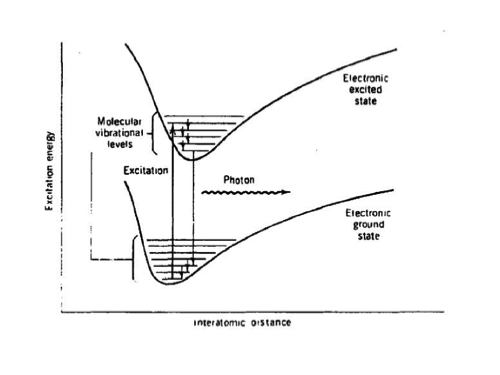
\includegraphics[width=15.0cm]{figures/Energy.png}
    \caption{Energy levels in plastic molecules.}
\label{fig:mol}
  \end{center}
\end{figure}


The light from the molecular deexcitation strikes a photocathode and release one or more photoelectrons per photon, called \textit{secondary electrons}, via Compton scattering. See Fig. \ref{fig:setup} for the experimental setup. The secondary electron are accelerated and multiplied in a photomultiplier tube (PMT) containing dynodes at different potential. The PMT hence produce an output voltage pulse, where the amplitude of the pulse is proportional to the number of scintillation events, which in turn is proportional to the energy deposited by the primary ionization. To keep this proportionality, the transparency mentioned earlier is necessary.  

The PMT only delivers a few electrons per event. The signal therefore needs to be amplified. Firstly, the signal is converted from a current to a voltage pulse in the preamplifier, with a typical size of $\sim mV$. Secondly, the pulse is amplified in the main amplifier, where the signal go from $\sim mV$ to $\sim V$. The pulse is then analyzed in he MCA, where it is digitized and stored in channels which can be displayed on a computer screen. 

To be able to translate the detected signal to the electron energy, the detector must be calibrated with the help of detecting radiation with known, discrete, energies from $^{207}Bi$ and $^{137}Cs$.  

\begin{figure}[htp]
  \vspace{40pt}
  \begin{center}
    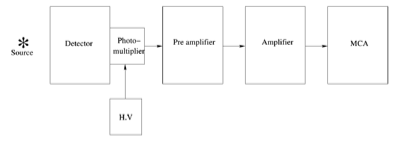
\includegraphics[width=15.0cm]{figures/Setup.png}
    \caption{The experimental setup.}
\label{fig:setup}
  \end{center}
\end{figure}



\section{The morning: measure $Q$ value of $^{32}$P}
Remember to save all the spectra!
\begin{enumerate}
\item Theory session 
\item Measure $^{207}Bi$ in 20 min for calibration of the detector -- measure two times: the second time with an Al-plate between the sample and the detector to stop the electrons 
\item Subtract the second spectrum from the total (left with only internal conversion, I.C., electrons with known energies)
\item Measure $^{137}Cs$ for 20 min
\item Calculate the weighted mean of the electron energies from I.C. by $<T>=\Sigma{(E\cdot I})/\Sigma{I}$, where $T$ is the electron energy, and $I$ the intensity, see Table \ref{tab:calib}
\item Calculate the calibration curve according to a straight line: $T_e=k\cdot ChNr+m$ 
\item  Measure $^{32}P$ for 1h 
\item Measure background for 1h and subtract background from $^{32}P$ electron spectrum
\item Construct the Fermi-Kurie plot by calculating the ingredients in $Q-T_e$ by -- preferable in Excel -- completing table \ref{tab:fkp}

\item Calculate the Q-value and compare to theory
\item Plot all spectra (using the data text file)

\end{enumerate}

\subsection{Data Analysis}
\label{sec:data-analysis}

\subsubsection{Prerequisites}
\label{sec:prerequisites}
\url{http://www.scipy.org/install.html}



\begin{table}[]
\caption{Electron energies}
\label{tab:calib}
\centering
\begin{tabular}{ccc}
Shell & $E_{e}$ (MeV) & I \\
$K_1$ & 0.483 & 1.55 \\
$L_1$ & 0.555 & 0.45 \\
$M_1$ & 0.568 & 0.15 \\
$K_2$ & 0.976 & 7.05 \\
$L_2$ & 1.049 & 1.85 \\
$M_2$ & 1.062 & 0.60 
\end{tabular}
\end{table}

\begin{table}[]
\caption{Ingredients in $Q-T_e$ (complete this table in Excel)}
\label{tab:fkp}
\centering
\begin{tabular}{|c|c|c|c|c|c|c|c|}
ChNr & $N(T_e)$ & $T_{e}$ (MeV) & $E_e$ (MeV) & $p$ (MeV/p) & $A$ & $f$ & $Q-T_e$ \\
1 & &  &  &  &  &  & \\
2 & From & From &  &  &  &See  & \\
. & data & calib- & quest & quest & $p/m_e$ & eq. \ref{eq:f} & $\sqrt{\frac{N(T_e)p}{E_ff}}$\\
. &  file & ration &  &  &  & \\
. &  &  &  &  &  &  & \\
1024 &  &  &  &  &  &  & 
\end{tabular}
\end{table}



\section{Preparatory questions}

\begin{enumerate}
\item Why is $^{32}P$ a suitable sample to use in this laboratory exercise?
\label{q:P}

\item How does the electron energy spectrum look like for a $\beta^-$ decay? Why? 
\label{q:cont}

\item Why must the proton undergoing $\beta^+$ decay be bound to a nucleus?
\label{q:+}

\item Can we treat $\beta^-$ as a point like interaction? Why? Hint: calculate the range the W-boson travels before it decay. The W mass is $\sim 80 GeV/c^2$. 
\label{q:point}

\item Calculate the Q-value for the process $^{32}P\rightarrow ^{32}S + e^- + \bar{\nu}$. Hint: you can neglect the neutrino mass and the difference in binding energy of the electrons, why? 

\item Write down the general expression for the matrix element $V_{fi}$. Optional: Write also the expression in the specific case of $\beta$ decay in terms of the wave functions. Hint: assume that the electron and neutrino are free particles after the decay; in addition we know that $pr<<1$ ($p$ is the electron momentum, and $r$ the radius).  
\label{q:V}

\item Why can we neglect all the constants in the derivation?
\label{q:const}


\item Why can we neglect the recoil energy of the daughter particle? 
\label{q:recoil}

\item Why is plastic a good material for a scintillator?
\label{q:plastic}


\label{q:q}
 
\end{enumerate}




\end{document}


